\section{Design der Controller}
\label{sec.Controller}
\subsection{Pendelidentifikation}
\label{Pendelidentifikation}
Beim Starten des Programmes zur Regelung des Pendels wird zunächst identifiziert, um welchen Pendelaufbau es sich handelt. Es wird dabei zwischen zwei zuvor definierten Pendelkonfigurationen unterschieden.
Für die Identifikation wird, nach einem kurzen Impuls durch den Motor, das Pendel frei schwingen gelassen, während der Controller den Verlauf von~$\theta_2$ aufzeichnet. Im Anschluss daran ist es möglich, aus den erhobenen Daten die Frequenz von~$\theta_2$ zu berechnen. Da sich die Frequenzen der Pendelkonfigurationen unterscheiden, kann das Programm so die entsprechenden Modelldaten laden und für die Regelung verwenden. In Abbildung \ref{fig.Identifikation} ist dieser Vorgang in den ersten fünf Sekunden zu erkennen.

\begin{figure}[htbp]
	\centering	
	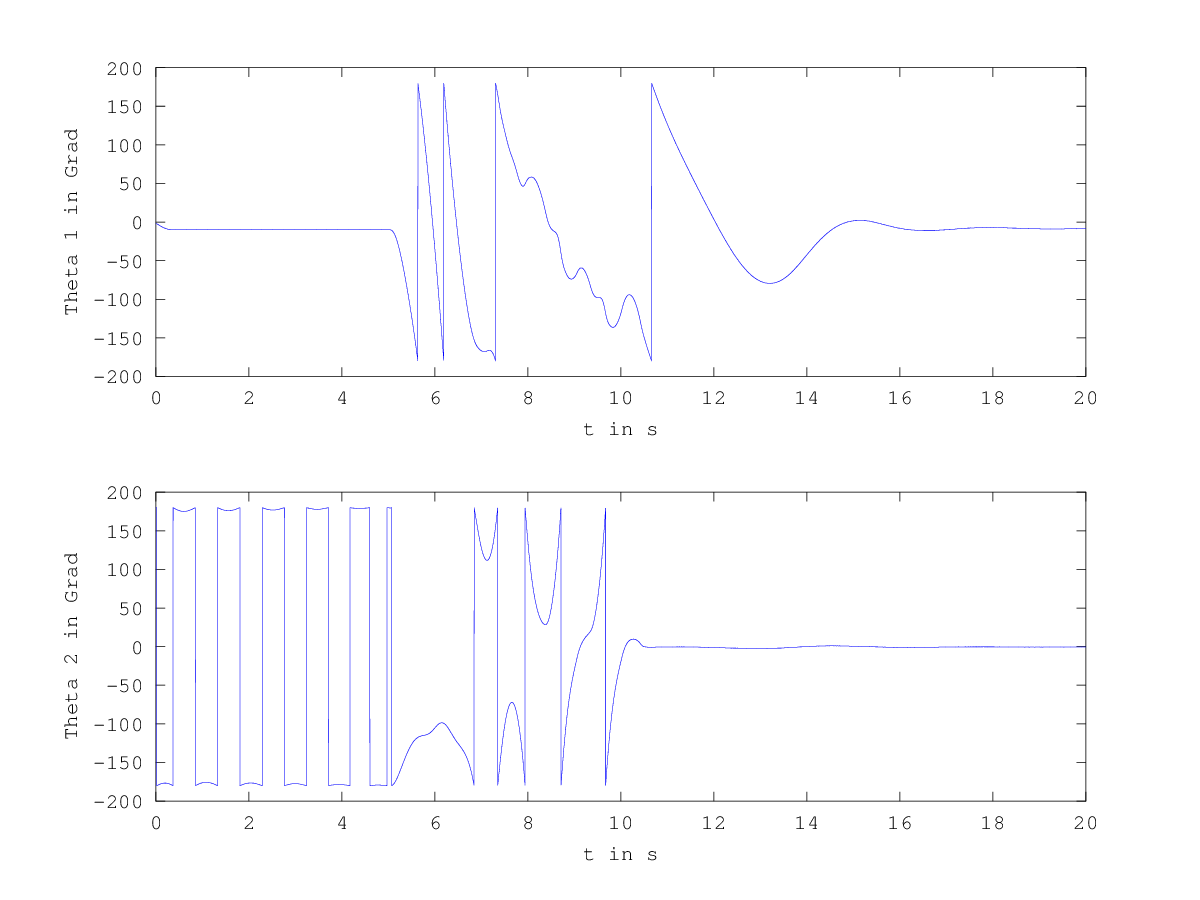
\includegraphics[width=0.8\textwidth]{Grafiken/Swingup_kurz.png}
	\caption{Initiale Pendelidentifkation}
	\label{fig.Identifikation}
\end{figure}


%\label{sec.Controller}
%\subsection{Signalverarbeitung}
%\label{signalverarbeitung} 
%Das Ausgangssignal der Inkrementalgeber wird zunächst auf Radiant-Werte umgerechnet 

\subsection{Swing-Up-Controller}
\label{Swing-Up-Controller} 

Der Swing-Up-Controller soll dem Aufschwingen des Pendels im Bereich $20^\circ < \left| \theta_2 \right| < 90^\circ$ dienen und basiert auf der Lyapunov-Funktion. Diese führt dazu, dass sich bei der Wahl von
$ \theta_2 = 0$ in der aufrechten Position des Pendels ein Regler ergibt, welcher die Energie des Pendels minimiert:

\begin{equation}
U_{SU} = n \cdot g \cdot sign(E-E_0)\dot{\theta}_2\cos(\theta_2)
\end{equation}

Der Term $E_0$ beschreibt die gewünschte, minimale Energie des Systems. Die Energie des Pendels $E$ setzt sich aus der potentiellen Energie $E_{pot}$ und der kinetischen Energie $E_{kin}$ zusammen. Die potentielle Energie lässt sich aufgrund der Referenz im höchsten Punkt des Pendels wie folgt berechnen:
\begin{equation}
E_{pot} = m_2 \cdot g \cdot l_2 \cdot (cos(\theta_2)-1)
\end{equation}

Die kinetische Energie ergibt sich zu:

\begin{equation}
E_{kin} = \frac{J_0}{2} \cdot \dot{\theta_2}^2
\end{equation}

Die Umsetzung des Reglers in Simulink ist in Abbildung \ref{fig.Simu_Swing-Up} zu sehen. 

\begin{figure}[h!]
  \centering	
  	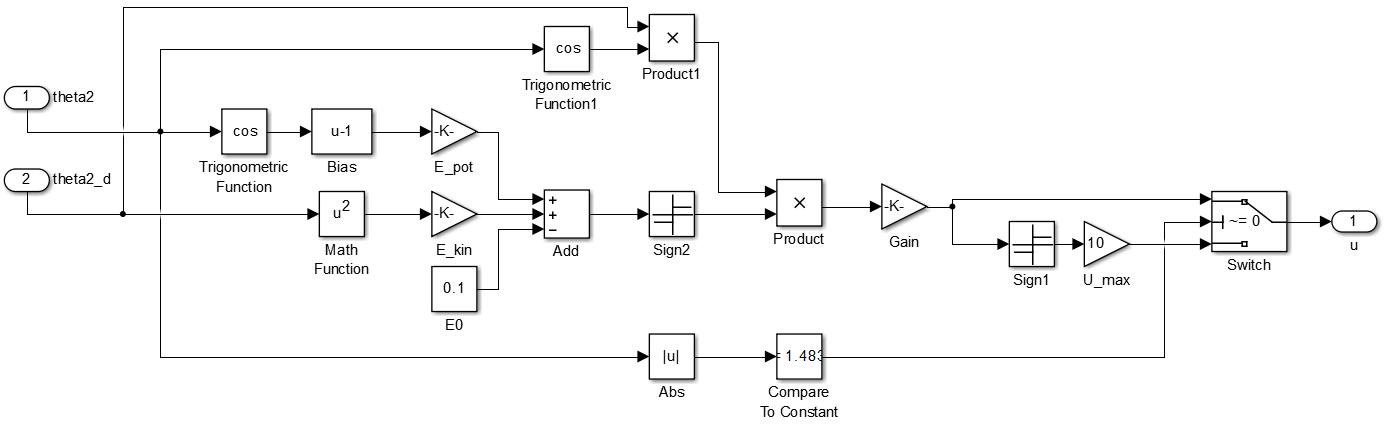
\includegraphics[width=1\textwidth]{Grafiken/simulink_swingup.png}
      \caption{Swing-Up-Controller und Zweipunktregler}
	\label{fig.Simu_Swing-Up}
\end{figure}


\subsection{Zweipunktregler}
\label{zweipunktregler} 

Für den Bereich $\left| \theta_2 \right| \geq 90^\circ$ soll ein Zweipunktregler (eng. Bang-bang control) das invertierte Pendel regeln. Dieser schaltet die maximale positive oder negative Spannung auf den Motor, abhängig von $ \theta_2 $ und $ \dot{\theta_2} $, daraus folgt die Übertragungsfunktion:

\begin{equation}
U = 10 \cdot sign(U_{SU} \cdot \theta_2 \cdot \cos(\dot{\theta}_2))
\end{equation}

Die Implementierung in Simulink ist ebenfalls als Teil des Modells in Abbildung~\ref{fig.Simu_Swing-Up} zu erkennen (Signum- und Gain-Baustein zusätzlich zum Swing-Up-Controller).


\subsection{Catcher}
\label{catcher} 

Der Catcher dient der genaueren Regelung des Pendels nahe des oberen Equilibriums von $ \theta_2 $. Um in dem Bereich optimal und robust zu Regeln, wird ein LQ-Regler verwendet. Dieser basiert auf der Minimiering der Cost-Function, welche folgenden Form besitzt:

\begin{equation}
 V = \int_0^\infty \! (x^T(t) Qx(t) + u^t(t) R u(t))  \mathrm{d}t
\end{equation}

Erhöht man die Diagonalwerte der Q-Matrix, werden die Fehler stärker Gewichtet, allerdings steigt auch der Aufwand der Regelung. Die Matrix lässt sich über die Controllability-Matrix $C$ und den linken Eigenvektor q der Matrix $A$
wie folgt berechnen:

\begin{equation}
 Q = C' \cdot q'^T \cdot q^T \cdot C
\end{equation}

Für den Vektor $q$ wurden folgenden Werte angenommen:

\begin{equation}
q =\begin{bmatrix}
         180/\pi/180 \\
         0\\
         0\\
         180/\pi/0.1
        \end{bmatrix}
\end{equation}
 
Die Diagonalwerte der Matrix R der Cost-Funktion beeinflussen die Geschwindigkeit der Regelung und wurden zunächst für den Catcher auf~$1$ gesetzt.
Zusammen mit den Eingangs- und Ausgangsmatrizen A und B lässt sich mithilfe des Matlab-Befehls $F = -lqr(A,B,Q,R)$ der LQR-Controller generieren.\citep{Werner.2013}

Die L-Matrix lässt sich über die Riccati-Gleichung herleiten, siehe \citep{Werner.2013}. Zunächst ergibt sich die P-Matrix als Lösung der Ricatti-Gleichung, daraus lässt sich mithilfe der bekannten Matritzen und des Place-Befehls $L=-place(A',C',p)'$ in Matlab berechnen.
Das Simulink-Modell des Observers ist in Abb. \ref{fig.obs_catcher} zu sehen.

\begin{figure}[htbp]
	\centering	
	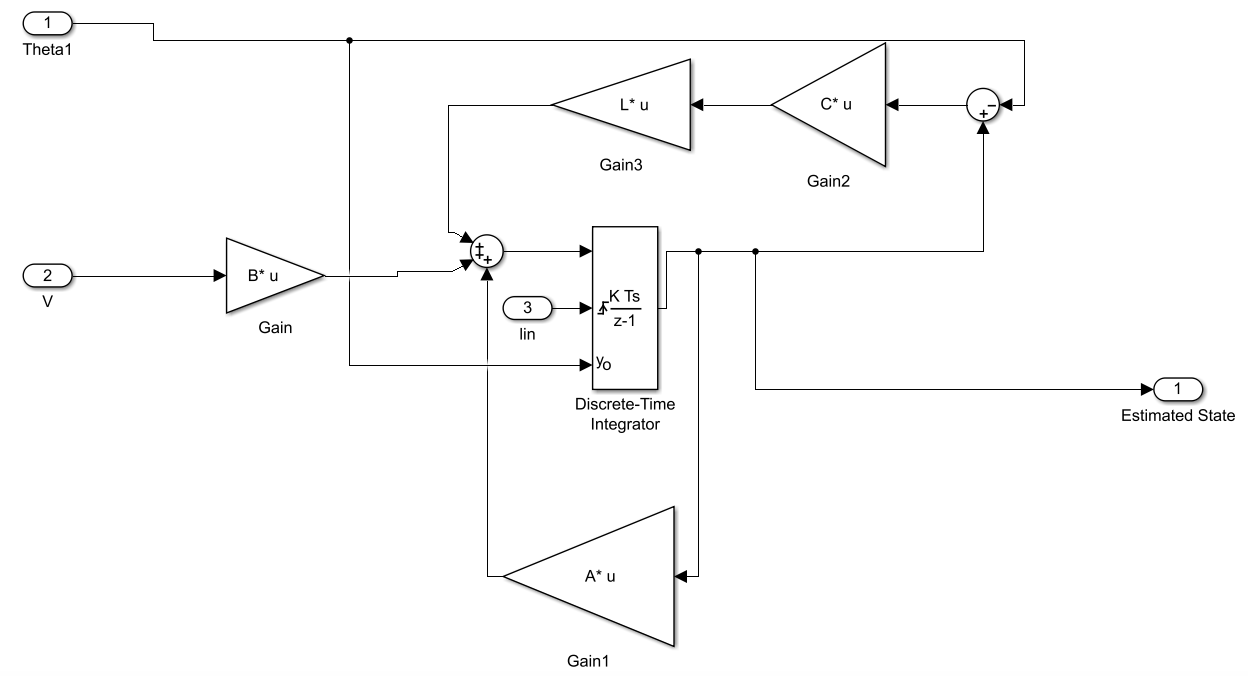
\includegraphics[width=0.8\textwidth]{Grafiken/simulink_observer_catcher.png}
	\caption{Observer des Catchers in Simulink}
	\label{fig.obs_catcher}
\end{figure}

\subsection{Stabilizer}
\label{stabilizer} 

Zur Rückführung des Pendels auf die Ausgangswinkel von $\theta_1$ und Beibehaltung der oberen Equilibrium-Position wird auch eine LQ-Regelung verwendet, welche sich nur durch die dreifache Einheitsmatrix für R und folgenden q-Vektor von dem Catcher unterscheidet:

\begin{equation}
q =\begin{bmatrix}
         180/\pi/1 \\
         0\\
         0\\
         180/\pi/0.1
        \end{bmatrix}
\end{equation}

Der Observer des Stabilizers ist in Abbildung \ref{fig.obs_stabilizer} dargestellt, während Abbildung \ref{fig.top_equilibrium} einen Überblick über die Verschaltung des Catchers und Stabilizers bietet.

\begin{figure}[htbp]
	\centering	
	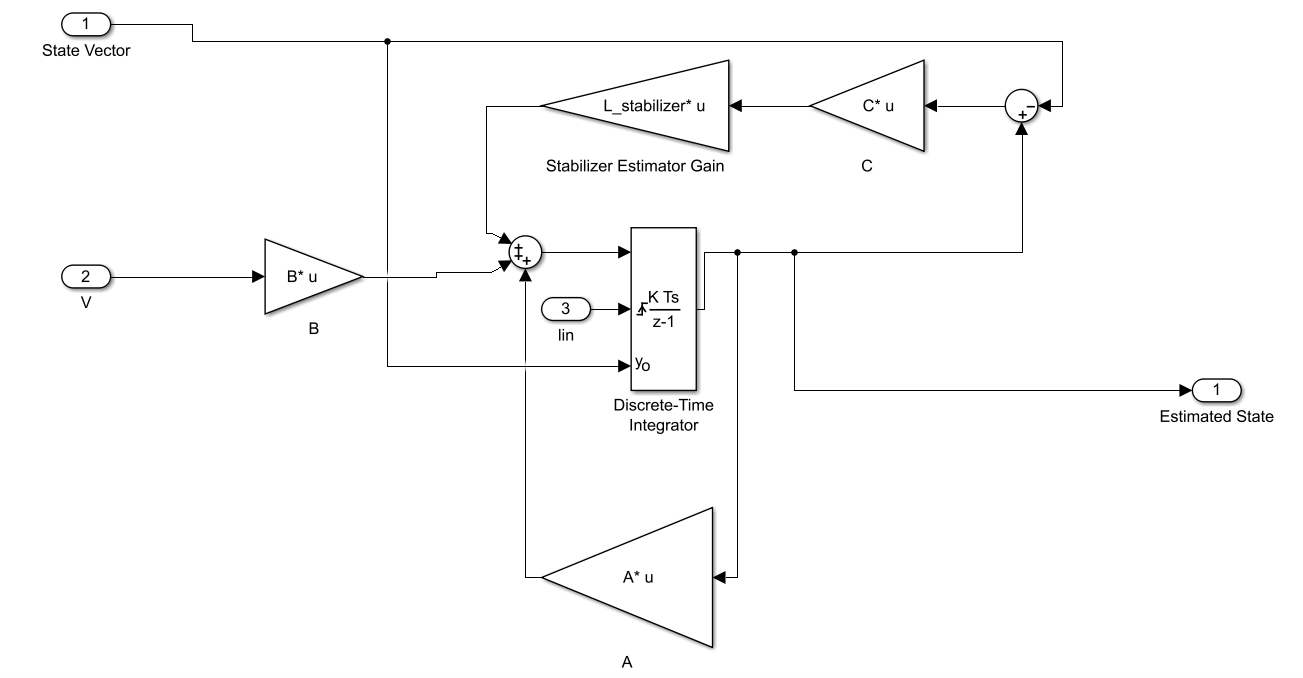
\includegraphics[width=1\textwidth]{Grafiken/simulink_observer_stabilizer.png}
	\caption{Simulink-Block des Observers des Stabilizers}
	\label{fig.obs_stabilizer}
\end{figure}

\begin{figure}[h!]
	\centering	
	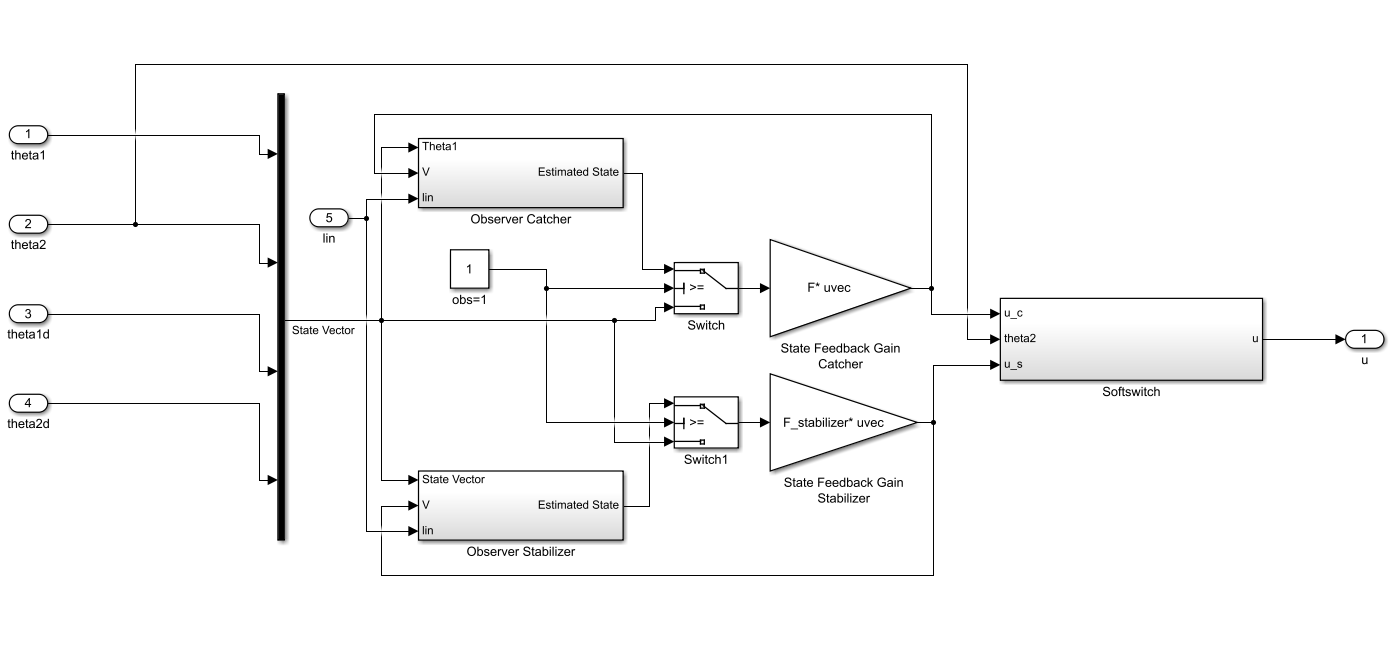
\includegraphics[width=1\textwidth]{Grafiken/simulink_top_equilibrium.png}
	\caption{Aufbau des Catchers und Stabilizers in Simulink}
	\label{fig.top_equilibrium}
\end{figure}

\subsection{Soft-Switch}
\label{Softswitch}
Um den Übergang zwischen dem Catcher und dem stabilisierenden Controller möglichst weich zu gestalten, wurde ein Soft-Switch implementiert.

Ziel dieses Switches ist es, extreme Sprünge des Controllerausgangssignals beim Umschalten zwischen den Controllern zu verhindern, selbst wenn die einzelnen Regelsignale des Catchers und des Stabilizers sehr weit auseinander liegen.

\begin{figure}[htbp]
	\centering	
	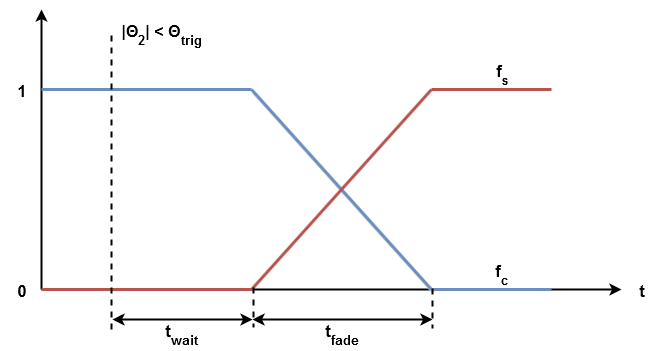
\includegraphics[width=0.8\textwidth]{Grafiken/SoftSwitch.png}
	\caption{Soft-Switch}
	\label{fig.Soft-Switch}
\end{figure}

Die Umsetzung erfolgt, indem die einzelnen Regelsignale mit Verstärkungsfaktoren multipliziert werden, die in der Summe genau~$1$ ergeben, und sich das Gesamtsignal aus den gewichteten Einzelsignalen zusammensetzt.

Zunächst ist lediglich der Catcher aktiv. Dies kommt dadurch zum Ausdruck, dass sein Verstärkungsfaktor $f_c$ den Wert 1 besitzt. Folglich muss der Faktor $f_s$ des Stabilizers 0 betragen.

Wenn nun der Betrag des Winkels $\theta_2$ für mindestens $t_{wait}$ kleiner als $\theta_{trig}$ ist, beginnt der Crossfader, das Verhältnis der Regelsignale zu verändern.
Während der Faktor des Catchers innerhalb der Zeit $t_{fade}$ linear von 1 auf 0 abfällt, erhöht sich der Faktor des Stabilizers gegenläufig innerhalb derselben Zeit von 0 auf 1.
Nach Abschluss dieses Vorgangs ist nur noch der Stabilizer für die Regelung des Pendels zuständig (vgl. Abbildung \ref{fig.Soft-Switch}). \\

Wird zu irgendeiner Zeit der Winkel $\theta_{trig}$ überschritten, wird augenblicklich mittels eines Hard-Switches der Catcher wieder aktiv geschaltet.

In unserem Controller wurden die Werte wie folgt gewählt:
\begin{eqnarray*}
&& \theta_{trig} = 5^{\circ} \\
&& t_{wait} = 0.5 s \\
&& t_{fade} = 5 s
\end{eqnarray*}

\begin{figure}[htbp]
	\centering	
	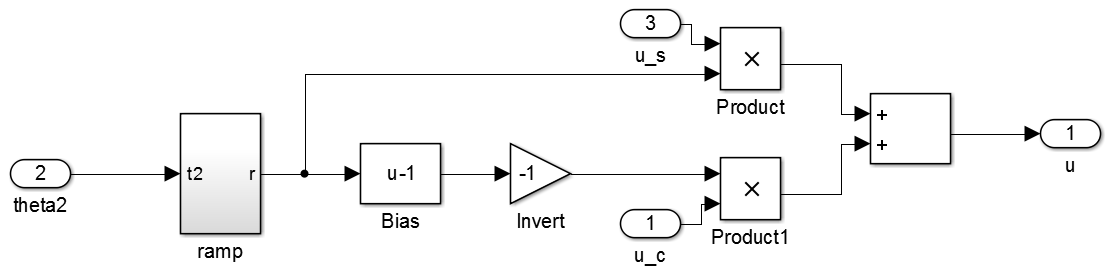
\includegraphics[width=0.8\textwidth]{Grafiken/simulink_softswitch.png}
	\caption{Soft-Switch in Simulink}
	\label{fig.Simu_Soft-Switch}
\end{figure}

Die Abbildung~\ref{fig.Simu_Soft-Switch} zeigt die Umsetzung dieses Soft-Switches in Simulink. Der Block `ramp' erzeugt dabei den Faktor $f_s$ woraus sich ebenfalls $f_c$ ableiten lässt.

Als Timer, wie sie innerhalb des `ramp' - Blocks zu finden sind, werden grundsätzlich Integrator-Blöcke verwendet. Schließt man am Eingang eines solchen Integrators die Konstante $1$ an, so ist der Wert des Ausgangs die Zeit seit dem letzten Reset.\\

\textit{Hinweis:} Die Funktionsweise dieses Verfahrens ist dabei identisch mit der eines Crossfaders, wie er teilweise beim Übergang zwischen zwei Musikstücken verwendet wird.

